\listfiles

% Dokumentenkopf
\documentclass[
    11pt, % Schriftgröße
    DIV=10,
    ngerman, % für Umlaute, Silbentrennung etc.
    a4paper, % Papierformat
    oneside, % einseitiges Dokument
    titlepage, % es wird eine Titelseite verwendet
    parskip=half, % Abstand zwischen Absätzen (halbe Zeile)
    headings=normal, % Größe der Überschriften verkleinern
    listof=totoc, % Verzeichnisse im Inhaltsverzeichnis aufführen
    bibliography=totoc, % Literaturverzeichnis im Inhaltsverzeichnis aufführen
    index=totoc, % Index im Inhaltsverzeichnis aufführen
    captions=tableheading, % Beschriftung von Tabellen unterhalb ausgeben
    numbers=noenddot,
    %draft % Status des Dokuments (final/draft)
    final % Status des Dokuments (final/draft)
]{scrreprt}

% Meta
\newcommand{\titel}{Konfiguration und Optimierung des Embedded-Linux-Betriebssystem für Automotive Image Processing Unit}
\newcommand{\untertitel}{Betreuer: Mladen Kovacev}
\newcommand{\art}{Bachelorarbeit}
\newcommand{\fachgebiet}{EDAG Engineering GmbH}
\newcommand{\autor}{Hugues landry Nseupi Nono}
\newcommand{\autorInit}{V.N.}
\newcommand{\addresse}{Salomon-Idler-Str 25}
\newcommand{\plz}{86159}
\newcommand{\ort}{Augsburg}
\newcommand{\telefon}{+49 157 79552970}
\newcommand{\mail}{landrynono60@yahoo.de}
\newcommand{\studienbereich}{Technische Informatik}
\newcommand{\matrikelnr}{2022666}
\newcommand{\pruefer}{Hubert Högl}
\newcommand{\jahr}{2022}
\newcommand{\logo}{images/FH-Augsburg-Logo.jpg}
\newcommand{\coverlogo}{images/FH-Augsburg-Logo-Text.jpg}

% Packages
% Anpassung des Seitenlayouts --------------------------------------------------
%   siehe Seitenstil.tex
% ------------------------------------------------------------------------------
\usepackage[
    automark, % Kapitelangaben in Kopfzeile automatisch erstellen
    headsepline, % Trennlinie unter Kopfzeile
    ilines % Trennlinie linksbündig ausrichten
]{scrlayer-scrpage}

% Anpassung an Landessprache ---------------------------------------------------
\usepackage[ngerman]{babel}

% Schrift ----------------------------------------------------------------------
\usepackage{lmodern} % bessere Fonts
\usepackage{relsize} % Schriftgröße relativ festlegen

% Umlaute ----------------------------------------------------------------------
%   Umlaute/Sonderzeichen wie äüöß direkt im Quelltext verwenden (CodePage).
%   Erlaubt automatische Trennung von Worten mit Umlauten.
% ------------------------------------------------------------------------------
\usepackage[utf8]{inputenc}
\usepackage[T1]{fontenc}
\usepackage{textcomp} % Euro-Zeichen etc.

% Grafiken ---------------------------------------------------------------------
% Einbinden von JPG-Grafiken ermöglichen

\usepackage[draft]{graphicx}
%\usepackage[dvips,final]{graphicx}
\DeclareGraphicsExtensions{.pdf,.png,.jpg,.eps}

% Befehle aus AMSTeX für mathematische Symbole z.B. \boldsymbol \mathbb --------
\usepackage{amsmath,amsfonts}

% für Index-Ausgabe mit \printindex --------------------------------------------
\usepackage{makeidx}

% Einfache Definition der Zeilenabstände und Seitenränder etc. -----------------
\usepackage{setspace}
\usepackage{geometry}

% Symbolverzeichnis ------------------------------------------------------------
%   Symbolverzeichnisse bequem erstellen. Beruht auf MakeIndex:
%     makeindex.exe %Name%.nlo -s nomencl.ist -o %Name%.nls
%   erzeugt dann das Verzeichnis. Dieser Befehl kann z.B. im TeXnicCenter
%   als Postprozessor eingetragen werden, damit er nicht ständig manuell
%   ausgeführt werden muss.
%   Die Definitionen sind ausgegliedert in die Datei "Glossar.tex".
% ------------------------------------------------------------------------------
\usepackage{siunitx}
\usepackage[intoc]{nomencl}
\let\abbrev\nomenclature
\renewcommand{\nomname}{Abkürzungsverzeichnis}
\setlength{\nomlabelwidth}{.25\hsize}
\renewcommand{\nomlabel}[1]{#1 \dotfill}
\setlength{\nomitemsep}{-\parsep}

% zum Umfließen von Bildern ----------------------------------------------------
\usepackage{floatflt}


% zum Einbinden von Programmcode -----------------------------------------------
\usepackage{listings}
\usepackage{xcolor} 

% URL verlinken, lange URLs umbrechen etc. -------------------------------------
\usepackage{url}

% wichtig für korrekte Zitierweise ---------------------------------------------
\usepackage[round]{natbib}

% PDF-Optionen -----------------------------------------------------------------
\usepackage[
    bookmarks,
    bookmarksopen=true,
    bookmarksnumbered, % nummerierte bookmarks im PDF
    colorlinks=true,
% diese Farbdefinitionen zeichnen Links im PDF farblich aus
    linkcolor=navy, % einfache interne Verknüpfungen
    anchorcolor=black,% Ankertext
    citecolor=navy, % Verweise auf Literaturverzeichniseinträge im Text
    filecolor=navy, % Verknüpfungen, die lokale Dateien öffnen
    menucolor=black, % Acrobat-Menüpunkte
    urlcolor=navy, 
% diese Farbdefinitionen sollten für den Druck verwendet werden (alles schwarz)
    %linkcolor=black, % einfache interne Verknüpfungen
    %anchorcolor=black, % Ankertext
    %citecolor=black, % Verweise auf Literaturverzeichniseinträge im Text
    %filecolor=black, % Verknüpfungen, die lokale Dateien öffnen
    %menucolor=black, % Acrobat-Menüpunkte
    %urlcolor=black, 
    backref,
    plainpages=false, % zur korrekten Erstellung der Bookmarks
    pdfpagelabels=true, % zur korrekten Erstellung der Bookmarks
    hypertexnames=true, % zur korrekten Erstellung der Bookmarks
    linktocpage % Seitenzahlen anstatt Text im Inhaltsverzeichnis verlinken
]{hyperref}
% Befehle, die Umlaute ausgeben, führen zu Fehlern, wenn sie hyperref als Optionen übergeben werden
\hypersetup{
    pdftitle={\titel \untertitel},
    pdfauthor={\autor},
    pdfcreator={\autor},
    pdfsubject={\titel \untertitel},
    pdfkeywords={\titel \untertitel},
}

% fortlaufendes Durchnummerieren der Fußnoten ----------------------------------
\usepackage{chngcntr}

% für lange Tabellen -----------------------------------------------------------
\usepackage{longtable}
\usepackage{array}
\usepackage{ragged2e}
\usepackage{lscape}
\usepackage{booktabs}
\usepackage{float}

% Spaltendefinition rechtsbündig mit definierter Breite ------------------------
\newcolumntype{w}[1]{>{\raggedleft\hspace{0pt}}p{#1}}

% Formatierung von Listen ändern -----------------------------------------------
\usepackage{paralist}

% bei der Definition eigener Befehle benötigt
\usepackage{ifthen}

% definiert u.a. die Befehle \todo und \listoftodos
\usepackage{todonotes}

% sorgt dafür, dass Leerzeichen hinter parameterlosen Makros nicht als Makroendezeichen interpretiert werden
\usepackage{xspace}

\usepackage{wrapfig}

\usepackage[labelfont=bf,font=small]{caption}
\captionsetup{format=plain} 

\usepackage{sidecap}

\usepackage{capt-of}

%\usepackage{needspace}

\usepackage{shorttoc} %\shorttableofcontents This package defines the \shorttableofcontents macro, which is used as follows: \shorttableofcontents{htitle i}{hdepth i} where htitlei will be the title of this table of contents and hdepthi its “depth”, with the meaning of the tocdepth counter.

\usepackage{lipsum}
\usepackage[strings]{underscore}

\usepackage{soul}

\usepackage{rotating}

% Erstellung eines Index und Abkürzungsverzeichnisses aktivieren ---------------
\makeindex
\makenomenclature

% Kopf- und Fußzeilen, Seitenränder etc. ---------------------------------------
% Zeilenabstand 1,5 Zeilen -----------------------------------------------------
\onehalfspacing

% Seitenränder -----------------------------------------------------------------
\setlength{\topskip}{\ht\strutbox} % behebt Warnung von geometry
\geometry{paper=a4paper,left=35mm,right=35mm,top=30mm}

% Kopf- und Fußzeilen ----------------------------------------------------------
\pagestyle{scrheadings}
% Kopf- und Fußzeile auch auf Kapitelanfangsseiten
\renewcommand*{\chapterpagestyle}{scrheadings} 
% Schriftform der Kopfzeile
\renewcommand{\headfont}{\normalfont}

% Kopfzeile
%\ihead{\large{\textsc{\titel}}\\ \small{\untertitel} \\[2ex] \textit{\headmark}}
\ihead{ ~\\~\\ \textit{\headmark}}
\chead{}
\ohead{}%\includegraphics[scale=0.15]{\logo}}
\setlength{\headheight}{21mm} % Höhe der Kopfzeile
% Kopfzeile über den Text hinaus verbreitern
\setheadwidth[0pt]{textwithmarginpar} 
\setheadsepline[text]{0.4pt} % Trennlinie unter Kopfzeile

% Fußzeile
\ifoot{}%\copyright\ \autor}
\cfoot{}
\ofoot{\pagemark}

% sonstige typographische Einstellungen ----------------------------------------

% erzeugt ein wenig mehr Platz hinter einem Punkt
\frenchspacing 

% Schusterjungen und Hurenkinder vermeiden
\clubpenalty = 10000
\widowpenalty = 10000 
\displaywidowpenalty = 10000

% Quellcode-Ausgabe formatieren
%\lstset{
%  frame=single,
%  basicstyle=\ttfamily\tiny,
%  numbers=left, 
%  numberstyle=\footnotesize, 
%  numbersep=5pt, 
%  breaklines=true, 
%  emph={square}, 
%  emphstyle=\color{red}, 
%  emph={[2]root,base}, 
%  emphstyle={[2]\color{blue}}}




% Fußnoten fortlaufend durchnummerieren
\counterwithout{footnote}{chapter}


\definecolor{bluegray}{RGB}{235,235,250}
\definecolor{colKeys}{rgb}{0,0,1}
\definecolor{colIdentifier}{rgb}{0,0,0}
\definecolor{colComments}{RGB}{108,226,108}
\definecolor{colString}{rgb}{0,0.5,0}
\definecolor{navy}{RGB}{0,0,128}
\definecolor{HSAorange}{RGB}{255,102,0}
\definecolor{HSAred}{RGB}{204,0,51}
\definecolor{dkgreen}{RGB}{0,100,30}
\definecolor{dkgray}{gray}{0.25}
\definecolor{gray}{gray}{0.5}
\definecolor{mauve}{rgb}{0.58,0,0.82}
\definecolor{orange}{RGB}{255,102,0}
\definecolor{lgGray}{gray}{1}
\definecolor{lstBg}{gray}{1}
\sethlcolor{lgGray}

% eigene Definitionen für Silbentrennung
% Trennvorschläge im Text werden mit \" angegeben
% untrennbare Wörter und Ausnahmen von der normalen Trennung können in dieser
% Datei mittels \hyphenation definiert werden

% listing config
% "define" Scala
\lstdefinelanguage{scala}{
  morekeywords={abstract,case,catch,class,def,%
    do,else,extends,false,final,finally,%
    for,if,implicit,import,match,mixin,%
    new,null,object,override,package,%
    private,protected,requires,return,sealed,%
    super,this,throw,trait,true,try,%
    type,val,var,while,with,yield},
  otherkeywords={=>,<-,<\%,<:,>:,\#,@},
  sensitive=true,
  morecomment=[l]{//},
  morecomment=[n]{/*}{*/},
  morestring=[b]",
  morestring=[b]',
  morestring=[b]"""
}

%\lstset{
%    float=hbp,
%    basicstyle=\ttfamily\color{black}\small,
%    identifierstyle=\color{colIdentifier},
%    %keywordstyle=\color{colKeys},
%    %stringstyle=\color{colString},
%    %commentstyle=\color{colComments},
%    keywordstyle=\color{blue},
%    commentstyle=\color{dkgray},
%    stringstyle=\color{dkgreen},
%    columns=flexible,
%    tabsize=2,
%    frame=single,
%    extendedchars=true,
%    showspaces=false,
%    showstringspaces=false,
%    numbers=left,
%    numberstyle=\tiny\color{gray},
%    breaklines=true,
%    backgroundcolor=\color{bluegray},
%    breakautoindent=true
%}
\lstset{
  basicstyle=\ttfamily\color{black}\footnotesize,
  numbers=left,               % Ort der Zeilennummern
  numberstyle=\tiny,          % Stil der Zeilennummern
  %stepnumber=2,               % Abstand zwischen den Zeilennummern
  numbersep=5pt,              % Abstand der Nummern zum Text
  tabsize=2,                  % Groesse von Tabs
  extendedchars=true,         %
  breaklines=true,            % Zeilen werden Umgebrochen
  numberstyle=\tiny\color{dkgray},
  keywordstyle=\color{blue},
  commentstyle=\color{orange},
  stringstyle=\color{dkgreen},
  frame=tb,
  %keywordstyle=[1]\textbf,    % Stil der Keywords
  %keywordstyle=[2]\textbf,    %
  %keywordstyle=[3]\textbf,    %
  %keywordstyle=[4]\textbf,   \sqrt{\sqrt{}} %
  %stringstyle=\color{white}\ttfamily, % Farbe der String
  showspaces=false,           % Leerzeichen anzeigen ?
  showtabs=false,             % Tabs anzeigen ?
  xleftmargin=0pt,
  framexleftmargin=2pt,
  framexrightmargin=2pt,
  framexbottommargin=0pt,
  backgroundcolor=\color{lstBg},
  showstringspaces=false      % Leerzeichen in Strings anzeigen ?
}

% eigene LaTeX-Befehle
% Eigene Befehle und typographische Auszeichnungen für diese

% einfaches Wechseln der Schrift, z.B.: \changefont{cmss}{sbc}{n}
\newcommand{\changefont}[3]{\fontfamily{#1} \fontseries{#2} \fontshape{#3} \selectfont}

\newcommand{\origttfamily}{}
\let\origttfamily=\ttfamily %Voheriges \ttfamily sichern
\renewcommand{\ttfamily}{\origttfamily \hyphenchar\font=`\-}

%highlighted texttt
\newcommand{\hltexttt}[1]{\texttt{\hl{#1}}}

% Abkürzungen mit korrektem Leerraum 
\newcommand{\Ua}{\mbox{U.\,a.\ }}
\newcommand{\ua}{\mbox{u.\,a.\ }}
\newcommand{\ZB}{\mbox{Z.\,B.\ }}
\newcommand{\zB}{\mbox{z.\,B.\ }}
\newcommand{\dahe}{\mbox{d.\,h.\ }}
\newcommand{\Vgl}{Vgl.\ }
\newcommand{\vgl}{vgl.\ }
\newcommand{\Bzw}{Bzw.\ }
\newcommand{\bzw}{bzw.\ }
\newcommand{\Bspw}{Bspw.\ }
\newcommand{\bspw}{bspw.\ }
\newcommand{\Evtl}{Evtl.\ }
\newcommand{\evtl}{evtl.\ }

\newcommand{\Uebs}[1]{Übs.: #1}
\newcommand{\uebs}[1]{übs.: #1}

\newcommand{\abbildung}[1]{Abbildung~\ref{fig:#1}}

\newcommand{\bs}{$\backslash$}

% erzeugt ein Listenelement mit fetter Überschrift 
\newcommand{\itemd}[2]{\item{\textbf{#1}}\\{#2}}

% einige Befehle zum Zitieren --------------------------------------------------
\newcommand{\Zitat}[2][\empty]{\ifthenelse{\equal{#1}{\empty}}{\citep{#2}}{\citep[#1]{#2}}}

% zum Ausgeben von Autoren
%\newcommand{\AutorName}[1]{\textsc{#1}}
\newcommand{\AutorName}[1]{{#1}}
\newcommand{\Autor}[1]{\AutorName{\citet*{#1}}}

% verschiedene Befehle um Wörter semantisch auszuzeichnen ----------------------
\newcommand{\Begriff}[1]{\textbf{#1}}
\newcommand{\Fachbegriff}[1]{\textit{#1}}

\newcommand{\Eingabe}[1]{\texttt{#1}}
\newcommand{\Code}[1]{\hltexttt{#1}}
\newcommand{\Datei}[1]{\texttt{#1}}

\newcommand{\Datentyp}[1]{\textsf{#1}}
\newcommand{\XMLElement}[1]{\textsf{#1}}
\newcommand{\Webservice}[1]{\textsf{#1}}


\newcommand{\footcite}[1]{\footnote{\citealp{#1}}}
\newcommand{\footuebscite}[2]{\footnote{\citealp{#1} \Uebs{#2}}}
\newcommand{\footvglcite}[1]{\footnote{\Vgl\citealp{#1}}}

\begin{document}
% Seitennummerierung -----------------------------------------------------------
%   Vor dem Hauptteil werden die Seiten in gr. römischen Ziffern nummeriert.
% ------------------------------------------------------------------------------
\pagenumbering{Roman}

% auch subsubsection nummerieren
\setcounter{secnumdepth}{3}
\setcounter{tocdepth}{3}

% Deckblatt und Abstract ohne Seitenzahl
\ofoot{}
\thispagestyle{plain}
\begin{titlepage}
  \thispagestyle{empty}  
  \addtolength{\textwidth}{55mm}
  \addtolength{\oddsidemargin}{-18mm}
  
  ~
  \begin{wrapfigure}{r}{25mm}
    \vspace{-40mm}
    \includegraphics[scale=0.4]{\coverlogo}
  \end{wrapfigure}
  
  
  \vspace{-1mm}
  
  \huge{\textcolor{HSAorange}{\fontfamily{phv}\selectfont\art}}
  
  
  \vspace{10mm}
  \Large{Studienrichtung \linebreak \studienbereich}
  \vspace{20mm}
  
  
  \begin{minipage}[t]{0.6\textwidth}
    \Large{\textbf{\titel}}\\[1.2ex]
    \large{\textbf{\untertitel}}\\
    \linebreak
    \large{in Kooperation mit der Firma: \fachgebiet}\\
    \linebreak
    \linebreak
    \large{Prüfer: \pruefer}\\
    
  \end{minipage}
  \hspace{0.1\textwidth}
  \hspace{5mm}
  \begin{minipage}[t]{40mm}
    \scriptsize
    Verfasser:\\
    \autor\\
    \addresse\\
    \plz\ \ort\\
    \telefon\\
    \mail\\
    Matrikelnr.: \matrikelnr\\
    
    \vspace{15mm}
    
    \textcolor{HSAred}{Hochschule für angewandte Wissenschaften Augsburg}\\
    \textcolor{HSAred}{An der Hochschule 1}\\
    \textcolor{HSAred}{86161 Augsburg}\\
    \textcolor{HSAred}{Telefon: +49 (0)821-5586-0}\\
    \textcolor{HSAred}{Fax: +49 (0)821-5586-3222}\\
    \textcolor{HSAred}{info@hs-augsburg.de}\\
    
  \end{minipage}
\end{titlepage}

\clearpage
\vspace*{\fill}



\begin{center}
	\copyright\ \jahr\ \autor \\
	
	\vspace*{15mm}
	
	Diese Arbeit mit dem Titel 
	
	">\titel\ -\ \untertitel"< 
	
	von \autor\ steht unter einer
	
	\textit{Creative Commons Namensnennung-Nicht-kommerziell-Weitergabe unter gleichen Bedingungen 3.0 Deutschland Lizenz} (CC BY-NC-SA). \linebreak
	\url{http://creativecommons.org/licenses/by-nc-sa/3.0/de/}
	
	
\includegraphics[scale=0.9]{images/CC_BY-NC-SA}
	
	\vspace*{15mm}
	
	Sämtliche, in der Arbeit beschriebene und auf dem beigelegten Datenträger vorhandene, Ergebnisse dieser Arbeit in Form von Quelltexten, Software und Konzeptentwürfen stehen unter einer GNU General Public License Version 3.\linebreak
	\url{http://www.gnu.de/documents/gpl.de.html}
	
	\vspace*{15mm}
	Die nachfolgende Arbeit enthält vertrauliche Informationen und Daten der Firma
EDAG Engineering GmbH.
	Veröffentlichungen oder Vervielfältigungen - auch nur auszugsweise oder in elektronischer
Form sind ohne ausdrückliche schriftliche Genehmigung der Firma EDAG Engineering GmbH
	nicht gestattet.

\end{center}


\vspace*{\fill}
\clearpage
\section*{sperrvermerk}
\label{sec:sperrvermerk}


\section*{Zusammenfassung}
\label{sec:Zusammenfassung}

Abstract auf Deutsch. Lorem ipsum dolor sit amet, consetetur sadipscing elitr, sed diam nonumy eirmod tempor invidunt ut labore et dolore magna aliquyam erat, sed diam voluptua. At vero eos et accusam et justo duo dolores et ea rebum. Stet clita kasd gubergren, no sea takimata sanctus est Lorem ipsum dolor sit amet. Lorem ipsum dolor sit amet, consetetur sadipscing elitr, sed diam nonumy eirmod tempor invidunt ut labore et dolore magna aliquyam erat, sed diam voluptua. At vero eos et accusam et justo duo dolores et ea rebum. Stet clita kasd gubergren, no sea takimata sanctus est Lorem ipsum dolor sit amet.

\section*{Abstract}
\label{sec:Abstract}

Abstract in English. Lorem ipsum dolor sit amet, consetetur sadipscing elitr, sed diam nonumy eirmod tempor invidunt ut labore et dolore magna aliquyam erat, sed diam voluptua. At vero eos et accusam et justo duo dolores et ea rebum. Stet clita kasd gubergren, no sea takimata sanctus est Lorem ipsum dolor sit amet. Lorem ipsum dolor sit amet, consetetur sadipscing elitr, sed diam nonumy eirmod tempor invidunt ut labore et dolore magna aliquyam erat, sed diam voluptua. At vero eos et accusam et justo duo dolores et ea rebum. Stet clita kasd gubergren, no sea takimata sanctus est Lorem ipsum dolor sit amet.
\ofoot{\pagemark}

%\phantomsection
%   \addcontentsline{toc}{chapter}{Kapitelverzeichnis} % Kapitelverzeichnis auch als Lesezeichen
%\shorttableofcontents{Kapitelverzeichnis}{0}

\pagebreak

\phantomsection
   \addcontentsline{toc}{chapter}{Inhaltsverzeichnis} % Inhaltsverzeichnis auch als Lesezeichen
\tableofcontents % Inhaltsverzeichnis

% Abkürzungsverzeichnis --------------------------------------------------------
\nomenclature{FPGA}{Field Programmable Gate Array}
\nomenclature{SOF}{Start of Frame}
\nomenclature{RTR}{Remote Transmission Request}
\nomenclature{DLC}{Data Length Code}
\nomenclature{CRC}{Cyclic Redundancy Check}
\nomenclature{PMU}{Platform Management Unit}
\nomenclature{CSU}{Configuration Security Unit}
\nomenclature{FSBL}{First Stage Bootloader Codes}
\nomenclature{CSU}{Configuration Security Unit}
\nomenclature{OCM}{On-Chip RAM}
\nomenclature{APU}{Application processing units}
\nomenclature{RPU}{Real-time processing units}

\nomenclature{CAN}{Control Area Network}
\nomenclature{IPU}{Image Processing Unit}


% für korrekte Überschrift in der Kopfzeile
\clearpage\markboth{\nomname}{\nomname}
\label{sec:Glossar}
\printnomenclature

\listoffigures % Abbildungsverzeichnis
%\listoftables % Tabellenverzeichnis
\renewcommand{\lstlistlistingname}{Verzeichnis der Listings}
\lstlistoflistings % Listings-Verzeichnis

% arabische Seitenzahlen im Hauptteil ------------------------------------------
\clearpage
\pagenumbering{arabic}

% Inhalt
\chapter{Einleitung}
\label{cha:Einleitung}

\section{Motivation}
\label{sec:Einl:Motivation}


\section{Ziel der Arbeit}
\label{sec:Einl:Ziel_der_Arbeit}



\section{Überblick über den Aufbau der Arbeit}
\label{sec:Einleitung:Aufbau_der_Arbeit}



\section{Typographische Konventionen}
\label{sec:Typographische_Konventionen}

Zum besseren Verständnis dieser Arbeit werden einige typographische Konventionen festgelegt.

Fachbegriffe werden \Fachbegriff{kursiv} formatiert.

Klassennamen und einzeilige Codefragmente werden in \Code{Proportionalschrift}, längerer Quelltext in Form von Codeblöcken, die als Listings bezeichnet werden, dargestellt.

Zitate und Metaphern werden in ">doppelte Anführungszeichen"< gestellt.

Liegt eine besondere Betonung auf einem Wort, so wird dieses \textbf{fettgedruckt} dargestellt.
Sonstige Hervorhebungen werden ebenfalls \textbf{fettgedruckt}.

Abkürzungen werden bei erster Nennung kurz erläutert und können zudem im Abkürzungsverzeichnis auf Seite \pageref{sec:Glossar} nachgeschlagen werden.
\clearpage

\chapter{Stand der Technik}
\label{cha:Stand_der_Technik}

Lorem ipsum dolor sit amet, consetetur sadipscing elitr, sed diam nonumy eirmod tempor invidunt ut labore et dolore magna aliquyam erat, sed diam voluptua. At vero eos et accusam et justo duo dolores et ea rebum. Stet clita kasd gubergren, no sea takimata sanctus est Lorem ipsum dolor sit amet. Lorem ipsum dolor sit amet, consetetur sadipscing elitr, sed diam nonumy eirmod tempor invidunt ut labore et dolore magna aliquyam erat, sed diam voluptua. At vero eos et accusam et justo duo dolores et ea rebum. Stet clita kasd gubergren, no sea takimata sanctus est Lorem ipsum dolor sit amet.
\section{First SoTA Chapter}
\label{sec:SoTA:first}

\begin{quote}
">Das Problem mit Zitaten aus dem Internet ist, dass man nie weiß ob sie echt sind."<
\citep{Einstein.2012}
\end{quote}

Lorem ipsum dolor sit amet, consetetur sadipscing elitr, sed diam nonumy eirmod \Fachbegriff{tempor} invidunt ut labore et dolore magna aliquyam erat, sed diam voluptua. At vero eos et accusam et justo duo dolores et ea rebum. Stet clita kasd gubergren, no sea takimata sanctus est Lorem ipsum dolor sit amet. Lorem ipsum dolor sit amet, consetetur sadipscing elitr, sed diam nonumy eirmod tempor invidunt ut labore et dolore magna aliquyam erat, sed diam voluptua. At vero eos et accusam et justo duo dolores et ea rebum. Stet clita kasd gubergren, no sea takimata sanctus est Lorem ipsum dolor sit amet.\footvglcite{Ipsum.2013}

Lorem ipsum dolor sit amet, consetetur sadipscing elitr, sed diam nonumy eirmod tempor invidunt ut labore et dolore magna aliquyam erat, sed diam voluptua (\vgl Abbildung~\ref{fig:hochschule}). At vero eos et accusam et justo duo dolores et ea rebum. Stet clita kasd gubergren, no sea takimata sanctus est Lorem ipsum dolor sit amet.

\begin{figure}
  \begin{center}
    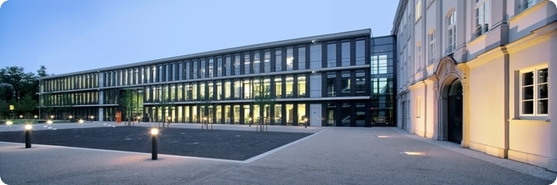
\includegraphics[width=0.6\textwidth]{./images/hochschule.jpg}
  \end{center}
  \vspace{-5pt}
  \caption[Hochschule Augsburg]{Hochschule Augsburg \cite{HSA.2013}} % Eckige Klammer (optional): Caption-Text in Abbildungsverzeichnis
  \label{fig:hochschule}
  \vspace{-5pt}
\end{figure}

\subsection{Unterabschnitt}
\label{subsec:SoTA:first:Unterabschnitt}

Lorem ipsum dolor sit amet, consetetur sadipscing elitr, sed diam nonumy eirmod \Fachbegriff{tempor} invidunt ut labore et dolore magna aliquyam erat, sed diam voluptua. At vero Abbildung~\ref{fig:standort_rotes_tor_anfahrt_klm_bau} eos et accusam et justo duo dolores et ea rebum.

\paragraph*{Beispiel}

\begin{wrapfigure}{r}{0.45\textwidth}
  \vspace{-20pt}
  \begin{center}
    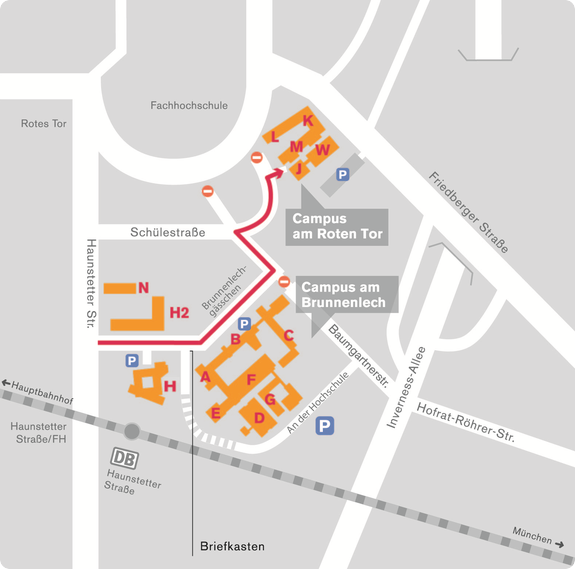
\includegraphics[width=0.45\textwidth]{./images/standort_rotes_tor_anfahrt_klm_bau.png}
  \end{center}
  \vspace{-20pt}
  \caption[Standort Rotes Tor]{Standort Rotes Tor \cite{HSA.2013}}
  \label{fig:standort_rotes_tor_anfahrt_klm_bau}
  \vspace{-10pt}
\end{wrapfigure}

Lorem ipsum dolor sit amet, consetetur sadipscing elitr, sed diam nonumy eirmod tempor invidunt ut labore et dolore magna aliquyam erat, sed diam voluptua. At vero eos et accusam et justo duo dolores et ea rebum. Stet clita kasd gubergren, no sea takimata sanctus est Lorem ipsum dolor sit amet. Lorem ipsum dolor sit amet, consetetur sadipscing elitr, sed diam nonumy eirmod tempor invidunt ut labore et dolore magna aliquyam erat, sed diam voluptua. At vero eos et accusam et justo duo dolores et ea rebum. Stet clita kasd gubergren, no sea takimata sanctus est Lorem ipsum dolor sit amet.

\begin{samepage}
  Lorem ipsum dolor sit amet, consetetur sadipscing elitr, sed diam nonumy eirmod tempor invidunt ut labore et dolore magna aliquyam erat, sed diam voluptua:
  \begin{description}
    \item[Lorem ipsum] dolor sit amet
    \item[consetetur] sadipscing elitr
    \item[diam nonumy] eirmod tempor invidunt
    \item[labore et dolore] magna aliquyam erat
  \end{description}
\end{samepage}

Mehr im Kapitel~\ref{sec:SoTA:second}.
\section{Second SoTA Chapter}
\label{sec:SoTA:second}

Lorem ipsum dolor sit amet, consetetur sadipscing elitr, sed diam nonumy eirmod tempor invidunt ut labore et dolore magna aliquyam erat, sed diam voluptua. 

\begin{itemize}
\item vero eos
\item accusam
\item justo duo dolores
\item ea rebum
\end{itemize}


Beispiel für Quelltexte (Siehe Listing~\ref{lst:HelloWorld}):

\begin{minipage}{\textwidth}
  \captionof{lstlisting}[Hello World]{Hello World \cite{coder.2009}} % Eckige Klammer (optional): Caption-Text in Listingsverzeichnis
  \vspace{-3pt}
  \begin{lstlisting}[language=java,label=lst:HelloWorld]
public class HelloWorld
{
  public static void main(String[] args)
  {
    System.out.println("HelloWorld");
  }
}
  \end{lstlisting}
\end{minipage}
\clearpage

\chapter{Fazit und Selbsteinschätzung}
\label{cha:Fazit_und_Selbsteinschaetzung}

Zuletzt soll dieses Kapitel neben einem kurzen Ausblick und einer Selbsteinschätzung auch noch ein Fazit bieten und damit die Arbeit abschließen.

\section{Ausblick}
\label{sec:FuS:Ausblick}

Lorem ipsum dolor sit amet, consetetur sadipscing elitr, sed diam nonumy eirmod tempor invidunt ut labore et dolore magna aliquyam erat, sed diam voluptua. At vero eos et accusam et justo duo dolores et ea rebum. Stet clita kasd gubergren, no sea takimata sanctus est Lorem ipsum dolor sit amet. Lorem ipsum dolor sit amet, consetetur sadipscing elitr, sed diam nonumy eirmod tempor invidunt ut labore et dolore magna aliquyam erat, sed diam voluptua. At vero eos et accusam et justo duo dolores et ea rebum. Stet clita kasd gubergren, no sea takimata sanctus est Lorem ipsum dolor sit amet.

\section{Selbsteinschätzung}
\label{sec:FuS:Selbsteinschaetzung}

Lorem ipsum dolor sit amet, consetetur sadipscing elitr, sed diam nonumy eirmod tempor invidunt ut labore et dolore magna aliquyam erat, sed diam voluptua. At vero eos et accusam et justo duo dolores et ea rebum. Stet clita kasd gubergren, no sea takimata sanctus est Lorem ipsum dolor sit amet. Lorem ipsum dolor sit amet, consetetur sadipscing elitr, sed diam nonumy eirmod tempor invidunt ut labore et dolore magna aliquyam erat, sed diam voluptua. At vero eos et accusam et justo duo dolores et ea rebum. Stet clita kasd gubergren, no sea takimata sanctus est Lorem ipsum dolor sit amet.

\section{Fazit}
\label{sec:FuS:Fazit}

Lorem ipsum dolor sit amet, consetetur sadipscing elitr, sed diam nonumy eirmod tempor invidunt ut labore et dolore magna aliquyam erat, sed diam voluptua. At vero eos et accusam et justo duo dolores et ea rebum. Stet clita kasd gubergren, no sea takimata sanctus est Lorem ipsum dolor sit amet. Lorem ipsum dolor sit amet, consetetur sadipscing elitr, sed diam nonumy eirmod tempor invidunt ut labore et dolore magna aliquyam erat, sed diam voluptua. At vero eos et accusam et justo duo dolores et ea rebum. Stet clita kasd gubergren, no sea takimata sanctus est Lorem ipsum dolor sit amet.


\clearpage


% Literaturverzeichnis ---------------------------------------------------------
%   Das Literaturverzeichnis wird aus der BibTeX "bibliography.bib" erstellt.
% ------------------------------------------------------------------------------
\bibliography{bibliography} % Aufruf: bibtex Masterarbeit
\bibliographystyle{natdin} %DIN-Stil des Literaturverzeichnisses
%\bibliographystyle{myplainnat} % custom


Ich, \autor, Matrikel-Nr.\ \matrikelnr, versichere hiermit, dass ich die vorliegende Arbeit mit dem Thema
\begin{quote}
\textit{\titel\ - \untertitel}
\end{quote}
selbständig verfasst und keine anderen als die angegebenen Quellen und Hilfsmittel benutzt habe, wobei ich alle wörtlichen und sinngemäßen Zitate als solche gekennzeichnet habe. Die Arbeit wurde bisher keiner anderen Prüfungsbehörde vorgelegt und auch nicht veröffentlicht.\\

\ort, den \today
\vspace*{1cm}\\
\rule[-0.1cm]{5cm}{0.5pt}\\
\textsc{\autor} 
 % Eidesstattliche Erklärung

% Anhang -----------------------------------------------------------------------
%   Die Inhalte des Anhangs werden in der Datei "Anhang.tex" inkludiert.
% ------------------------------------------------------------------------------
\begin{appendix}
    \clearpage
    \pagenumbering{alph}
    \chapter{Anhang}
    \label{sec:Anhang}
    % Rand der Aufzählungen in Tabellen anpassen
    \setdefaultleftmargin{1em}{}{}{}{}{}
    \section{Inhalt des Datenträgers}
\label{apx:Datentraeger}

Der dieser Arbeit beigelegte Datenträger beinhaltet zusätzliche Materialen. 
Neben der Arbeit selbst im Portable Document Format (PDF) befinden sich sowohl die Sources der Implementierungen als auch die lauffähigen Pakete.

\begin{description}
\item[\texttt{./all-my-packages/}] ~ \linebreak 
\noindent\hspace*{10mm} Sources der Packages
\item[\texttt{./Architektur/}] ~ \linebreak 
\noindent\hspace*{10mm} UML-Diagramme der Architektur
\item[\texttt{./Thesis\_Vorname\_Nachname\_123456.pdf}] ~ \linebreak 
\noindent\hspace*{10mm} PDF Version dieser Arbeit
\item[\texttt{./ThesisVM.ova}] ~ \linebreak 
\noindent\hspace*{10mm} Virtual Box Image mit lauffähiger Demoumgebung
\end{description}
\end{appendix}

% Index ------------------------------------------------------------------------
%   Zum Erstellen eines Index, die folgende Zeile auskommentieren.
% ------------------------------------------------------------------------------
%\printindex


\end{document}
